%%%%%%%%%%%%%%%%%%%%%%%%%%%%%%%%%%%%%%%%%%%%%%%%%%%%%%%%%%%
% EPFL report package, main thesis file
% Goal: provide formatting for theses and project reports
% Author: Mathias Payer <mathias.payer@epfl.ch>
%
% To avoid any implication, this template is released into the
% public domain / CC0, whatever is most convenient for the author
% using this template.
%
%%%%%%%%%%%%%%%%%%%%%%%%%%%%%%%%%%%%%%%%%%%%%%%%%%%%%%%%%%%
\documentclass[a4paper,11pt,oneside]{report}
% Options: MScThesis, BScThesis, MScProject, BScProject
\usepackage[MScProject]{EPFLreport}
\usepackage{xspace}

\usepackage{graphicx}
\usepackage{times}
\usepackage{fancyhdr,graphicx,amsmath,amssymb}
\usepackage{multirow}
\usepackage[ruled,vlined]{algorithm2e}
\include{pythonlisting}

\title{Resilient Deniable Storage}
\author{Andrej Milicevic}
\supervisor{Dr. Vero Estrada-Gali\~{n}anes}
% \adviser{Prof. Dr. sc. ETH Mathias Payer}
%\coadviser{Second Adviser}
% \expert{The External Reviewer}

\newcommand{\sysname}{FooSystem\xspace}

\begin{document}
\maketitle
% \makededication
\makeacks

\maketoc

%%%%%%%%%%%%%%%%%%%%%%
\chapter{Introduction}
%%%%%%%%%%%%%%%%%%%%%%

Plausible deniability, in the context of data storage, is a cryptographic primitive which involves creating a situation where the existence or presence of certain data is not easily verifiable or provable. The goal is to provide individuals with the ability to deny the existence of sensitive or private information, even if it is present within their data storage systems. While backups of such data should be created, in certain use cases, such as data being exfiltrated, this is not possible. That is where we can add a redundancy scheme which will recover from some data corruption, and prevent as much loss as possible. 

This powerful cryptographic primitive is a good way of ensuring coercion resistance. Data coercion describes unauthorized or malicious data manipulation, typically with the intent to gain unauthorized access, or extract some sensitive information from the system. Therefore, coercion resistance focuses on designing storage systems such that they are resistant to coercion attempts. 

In this report, we will look into implementing a redundancy scheme called a \emph{simple entanglement}, which will work on an arbitrary block device. Afterwards, we will use this scheme along with a coercion-resistant tool called \emph{Shufflecake}. The aim is to increase the resilience of said tool. The scheme is implemented as a device-mapper target for the Linux kernel (version 6.2). 

The next section describes Shufflecake in more detail. This is followed by the description of simple entanglements in section 3 and the details of the implementation in section 4. Section 5 discusses the usage of the tool presented in this report, and how entanglements are used together with Shufflecake. Finally, the results of this implementation, as well as further steps for this project are presented in the last two sections. 

I did a lot of the research regarding the Linux kernel, block device drivers, device-mapper targets, and similar topics with the help of two books: \emph{Linux Device Drivers} \cite{ldd3}, and \emph{Linux Kernel Development} \cite{love2010linux}. 

\chapter{Shufflecake}
Shufflecake is a tool used to create multiple hidden volumes on a storage device. It is a successor to tools such as TrueCrypt and VeraCrypt, and provides two key properties that those tools do not: Shufflecake can create multiple hidden volumes, not just one, and it is independent of the filesystem of the underlying storage device. 

Shufflecake is designed as a device-mapper target for the Linux kernel. The current version has been tested with kernel versions 6.1, 6.2, and 6.3. Shufflecake can handle creating up to 15 hidden volumes on one storage device. The device storage space is divided into two parts: the header section, and the data section. The header section contains metadata for all volumes which are created, divided into a header for each volume. There is always enough reserved space for the maximum number of volumes, irrespective of the actual number of created volumes. This is simply to keep the number of volumes secret. 

The data section is further comprised of sections of contiguous blocks, called \emph{slices}. When using the volumes, the user interacts with logical slices, and these are allocated as needed. When a user requests a block of memory, a whole logical slice is allocated (if it has not been allocated already), and the contents are written to the physical storage space, in the form of a physical slice. The physical slices are randomly interleaved on disk, therefore there is no static correspondence between the logical and physical slice indices. Because of this randomness, each volume has a slice map in its header, mapping the index of the logical slice to the index of its physical slice. How these slices look can be seen in Figure \ref{fig:shufflecake-slices}.

\begin{figure}[!ht]
    \centering
    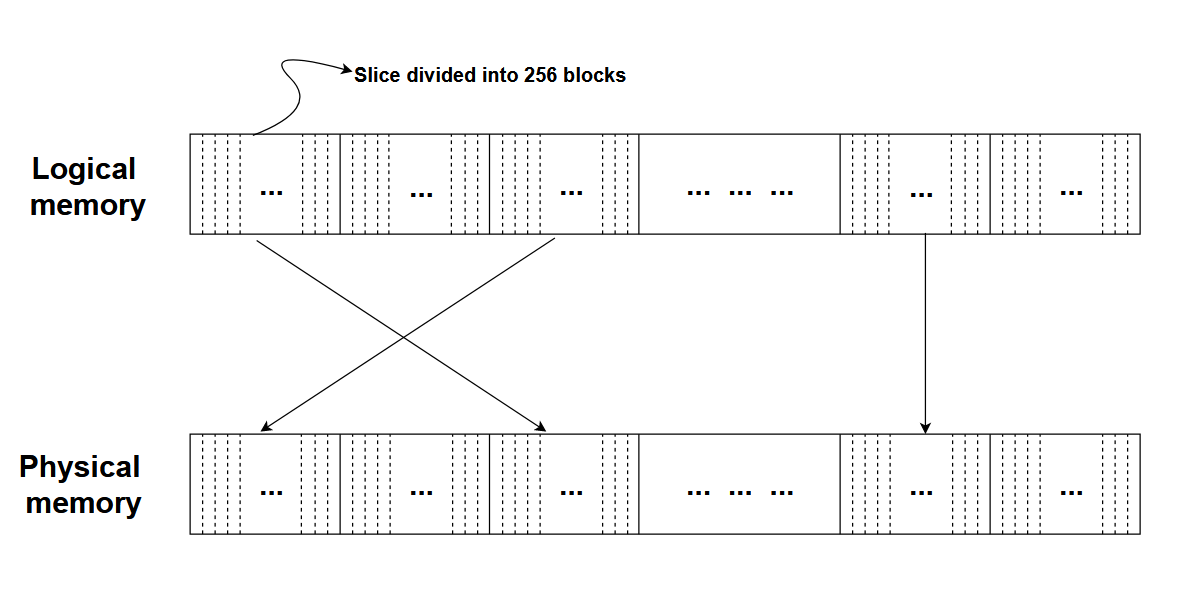
\includegraphics[scale=0.5]{figures/Shufflecake-slices.PNG}
    \caption{Arrangement of logical and physical slices in Shufflecake}
    \label{fig:shufflecake-slices}
\end{figure}

While this tool is an improved version of its predecessors, it still has its own flaws, one of them being the very real possibility of data corruption. Since each volume appears to have the full capacity of the underlying storage device at its disposal, a user could overcommit resources and overwrite data which looks like free memory, but is actually just hidden. Since there are no solutions to this implemented in the original Shufflecake, the user must be cautious when using it, and should follow the guidelines provided by the authors, such as opening all volumes when "home alone", regardless of which volumes they will use. Data corruption is, however, unavoidable in the case of the user being "under investigation", therefore with this project we attempt to mitigate the corruption as much as possible. 

For more details on Shufflecake, the reader is directed to the original paper by Elia Anzuoni, "Hidden Filesystem Design and Improvement" \cite{elia}, and also the source code of the tool, which can be found on Codeberg.org \cite{shufflecake-code}. 

\chapter{Redundancy scheme}

As it is explained in the original paper \cite{elia}, and tested in previous work \cite{kilian}, the corruption of data when using Shufflecake could be substantial. If the user does not open all volumes, as suggested by the authors, they risk corrupting any important files they have on hidden volumes. The more storage space is used, the higher the chance of data corruption, and the growth of said corruption is not necessarily linear, as shown in \cite{kilian}. When under investigation, it is assumed that the investigator can do whatever they want, hence even if the user is careful when they use Shufflecake, this data corruption might still happen. To this end, some mitigations have already been implemented. These mitigations include using readily available tools, such as \texttt{mdadm} \cite{mdadm_man}, a Linux tool to create and monitor RAID partitions, and also integrating RAID-like mirroring in Shufflecake itself, on a slice-level granularity \cite{kilian}. As a continuation of this work, we will attempt to resolve some issues that are still left open regarding adding redundancy to this tool. 

In order to keep the original philosophy of Shufflecake, we will work on adding redundancy within each volume, thus keeping the secrecy hierarchy intact. We will not use mirroring, but rather simple entanglements \cite{estrada}, a more reliable approach to redundancy. Simple entanglements will be discussed in detail in the following subsection. Since Shufflecake works with 4096-byte blocks as the smallest unit of I/O, this implementation will also consider such blocks, and entanglements will be implemented at the block granularity. Why we chose to do so is described in more detail in section 3.2. 

\section{Simple entanglements}
Simple entanglements represent data distributions for log-structured append-only storage systems. We have two types of such entanglements: open and closed entanglements. They both work in the same way: for each \emph{data block}, we create and store a \emph{parity block}. We do create space overhead, however it is the same overhead as with mirroring. The main component of this scheme is the entanglement chain, which is comprised of data and parity blocks connected together in an alternating manner, as seen in Figure \ref{entanglement}. The parities are computed using the XOR operation between the previous two elements in the entanglement chain. 

\begin{figure}[!ht]
    \centering
    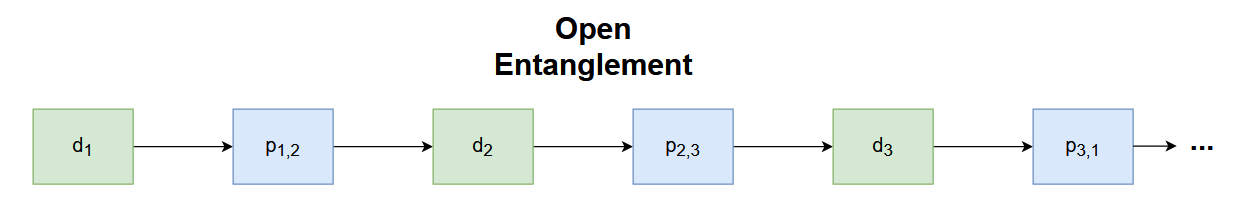
\includegraphics[scale=0.5]{figures/Open_entanglement.PNG}
    \caption{Example of an open entanglement}
    \label{entanglement}
\end{figure}

If we take the parity block $p_{2,3}$ as an example, it was calculated by doing the XOR operation between the parity block $p_{1,2}$ and the data block $d_{2}$. The entanglement follows in a similar fashion along the chain. 

Due to the properties of the XOR operation, recalculating (i.e. repairing) blocks which have been corrupted is easy. Continuing the previous example, in case data blcok $d_{2}$ is corrupted, we can recalculate it by XOR-ing the two adjacent parity blocks, $p_{1,2}$ and $p_{2,3}$. For corrupted parity blocks, we have two choices. Take parity $p_{2,3}$ as an example. We can recalculate it by XOR-ing either $p_{1,2}$ and $d_{2}$, or $d_{3}$ and $p_{3,4}$. 

In this implementation, we will work on adding redundancy within a single Shufflecake volume, i.e. implementing the scheme to work on top of an arbitrary block device. 

We will implement an open entanglement, meaning that there is no connection between the last and first member of the chain. Since we have an open entanglement in our case, we have three particular types of failures to look out for. If any of these cases happen, the blocks involved are irrecoverable. As seen in Figure \ref{fig:irrecoverable_failures}, these failures are called type A, type B, and type C. Type A refers to the situation if both the last data and parity blocks get corrupted: both of these blocks are irrecoverable in that scenario. Type B refers to a failure of two consecutive data blocks, and the parity block between them. Finally, type C describes the situation where two data blocks and all parity blocks between them fail. All these failures result in some blocks being lost forever. 

\begin{figure}[!ht]
    \centering
    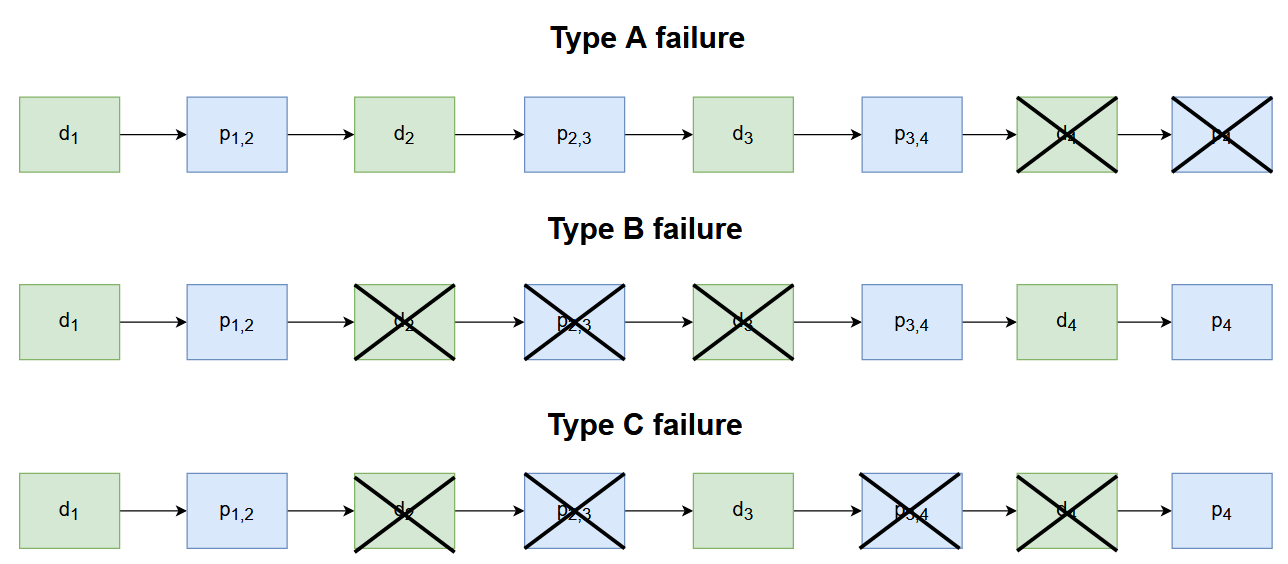
\includegraphics[scale=0.5]{figures/Irrecoverable_failures.PNG}
    \caption{The 3 types of failures where some blocks are irrecoverably lost.}
    \label{fig:irrecoverable_failures}
\end{figure}

In case of a user deleting files, we do not do anything special. The blocks will be reused in the future for new files, however there exists an issue here. When reusing a block that was already in the entanglement, we would need to recalculate the entire entanglement all over again, since we changed the contents of a block possibly in the middle of the entanglement. While this poses a serious limitation, this is due to the nature of the simple entanglements, since they represent a data distribution layout for \emph{append-only} storage systems. 

For further reading and a more detailed explanation of simple entanglements, the reader is directed to the original paper, "Simple Data Entanglement Layouts with High Reliability". \cite{estrada}.

\section{Granularity of the implementation}
Before actually implementing this scheme, we need to determine the granularity at which we will do so. Naturally, the first idea is to work with slices within Shufflecake. For every slice, we create a parity, and save everything in storage. This idea, however, does not work well, and the main reason for that is the fact that slices can be reused in the following way. A slice is 1MB in size, and when a user, for example, creates a file of size 100KB, a whole slice is allocated, but the rest of it can later be used by other user requests. Shufflecake tries to use slices as much as possible, and only allocates new ones when necessary. If we were to use the slice in our entanglement calculation, and that slice is later reused, a recalculation of the whole entanglement chain would be necessary. All this can be avoided by just implementing the entanglement on the 4KB block level. We create a parity block for each data block, XOR them to create new parities, and then repair any corruption block by block. 

Since we are changing the granularity, we also need a way to check for data corruption at the block level. In the case of slices, we could check if a slice was allocated more than once, indicating that some data had been overwritten, and thus corrupted. This, however, does not work in our case. The simplest solution for this is to use checksums. A checksum is calculated for each block, and saved to storage so that it can be verified when needed. More details on this, as well as other metadata and the storage overhead they produce, in section 4.2. 

\chapter{Implementation details}
In this section, all implementation details are presented, starting from the first ideas, why they were abandoned, and how this scheme is finally implemented.

\section{Continuing previous work}
Naturally, the first idea was to look at the work previously done on this problem \cite{kilian}, and to try and build upon the solutions that were presented then. These involved implementing a RAID-like redundancy scheme on Shufflecake volumes, and some of the problems the author encountered were regarding the filesystem metadata which is persisted in storage. The filesystem in question was the ext4 filesystem, as the most widely used Linux filesystem. The redundancy scheme seemed to overwrite some filesystem metadata, such as superblocks, which then caused a total crash of the filesystem. My first idea was to look into the details of the ext4 filesystem, and try to avoid such crashes. 

After some research, and a few conversations I had with the creators of Shufflecake, Elia Anzuoni and Dr. Tommaso Gagliardoni, this idea was quickly abandoned. The reason being that Shufflecake is independent of any filesystem, thus tailoring a solution specifically for ext4 does not seem logical. A better way to implement this scheme is to create a block device driver, or a new device-mapper target for the Linux kernel. Thus, I did more research into block device drivers, and how this redundancy scheme would work in that case. After some time, and a talk with Elia, we figured that this was not a good solution, since creating new block device drivers is unnecessarily complicated in this scenario. Therefore, the conclusion was that the device mapper target is the way to go, and that a block device driver is not needed in this case. This new kernel module would take care of the entanglement chain, and all the necessary details needed to make it work. If we have that, then the module can be loaded into the kernel, and Shufflecake could use it as a sort of black box, without knowing any implementation details. 

More on how this new module could be incorporated into Shufflecake in section 5. The following subsections explain how this device-mapper target achieves the goal of redundancy and implements the entanglement chain of blocks. 

\section{Creating and writing blocks}
Since the entanglement is implemented as a device mapper target, the way we write blocks is simple: we intercept the write requests, called \emph{bio} requests. For each 4KB data block intercepted, we calculate the parity block, and store both blocks on the underlying device. The way we differentiate between data and parity blocks is by their address, called sector number. The first half of the underlying device contains data blocks, while the other half contains parities. When we intercept the write request, we can calculate the sector for the parity block, create a new request for that parity, and submit both the data and parity requests to the layer below, where the blocks will be persisted to disk. The reason we store data blocks first, and then parities, is to avoid corrupting sensitive blocks, such as filesystem metadata. This way, we essentially act as tho we have two drives, the first one containing actual data, and the other containing parity blocks. 

When calculating the new parity blocks, we do have to pay attention to how this is done. Since we always need the last block in the entanglement chain, we should keep it cached in memory, to avoid doing a read operation for every write. This would create unnecessary overhead. This cached block is updated every time we write new blocks. 

We also intercept read requests. For such requests, we can just submit them to the device, since we do not change the sector of a data block when intercepting write requests. 

\section{Block metadata}
Another part of this implementation is keeping the metadata that we need persisted on the disk. Firstly, since the allocation of blocks by upper layers (e.g. when a user creates files) is random, we need to save the information about how the blocks are entangled. This is done by saving the sectors of blocks in the order in which they appear in the entanglement chain. Therefore, for each block, we use additional 8 bytes of memory to keep the sector, which is of the data type \texttt{long}. More specifically, we save the logical sector. Since we work on 4KB blocks as the basic unit of I/O, and the Linux kernel works with 512-byte blocks, we need to differentiate between two different sectors. In this case, we only care about logical sectors because we are working with 4KB blocks. Due to this, it is necessary to scale the sector accordingly when submitting a read or write operation. For example, a block at logical sector 100 would be at the physical sector 800, since the basic I/O units are of different sizes. 

Since we are creating a mechanism to mitigate data corruption, we need a way to check if a block has been corrupted. This is done by calculating a CRC32 checksum for each block, and saving it in storage. Similarly to the block sectors, we persist the checksums (the blocks containing checksums start after the block containing the entnaglement chain). In fact, there is a static correspondence between the saved entanglement and the checksums: first checksum corresponds to the first sector, second checksum to the second sector, etc. For the checksums, additional 4 bytes of memory is used per block.

In summary, we use 12 bytes per 4096-byte block (by block here, we mean both data and parity blocks) to store all the information we need to implement this mechanism. This is a less than $0.3\%$ storage overhead. 

The reason I save the metadata after the user data, as seen on Figure \ref{fig:volumes-diagram} is simply an implementation detail. Some functions from a library used for device mapper targets did not work quite as I had hoped, so I had to find a workaround. It does not change the implementation in any significant way, other than the fact that the metadata is accessed via different addresses (i.e. sectors). 

\section{Loading and storing the entanglement}
We talked about storing the entanglement chain and the block checksums in storage, but we also need to know how and when to write/read that information to/from the disk. 

Ideally, we would update the storage every time we introduce new blocks, to have the most consistency possible in the event of a crash. However, since we only persist sectors and checksums, which are fairly small values in terms of bytes, it would be wasteful to do so. The reason is the following: the smallest unit of I/O in our case is a 4096-byte block, meaning that in order to persist the metadata for two new blocks that come on every write (data block and parity block), we would need to update a metadata block. This would cause a read of the metadata block currently being updated, and then the write of that block when we update its contents. This is far too wasteful in terms of I/O. Instead, we keep two buffers, one for sectors and one for checksums, and update them with every write request. Their size is the size of a block, 4KB, and when they are full, we flush them to storage. Thus, we have eliminated the potential waste of I/O. 

In the case of loading the information from storage, we do it when our module is loaded in the kernel. We create a list of blocks to represent the entanglement chain, and we create a map for the checksums. We map each sector with its checksum, that way it will be easier and faster to check for data corruption. 

\section{Checking for corrupted blocks}
The search for corrupted blocks is simple: we go through all blocks, checking if the checksum of the current block matches with the checksum of when that block was written to disk. If not, we found a corrupted block, and we flag it. We keep a bitmap which says if a block has been corrupted or not. One bit for each block sector, i.e. each block. The bit is 0 if the block is good, 1 if it is corrupted. 

\section{Repairing corrupted blocks}
Once we find which blocks have been corrupted, we need to repair them, if we can. While we conduct the repair, we mark the blocks which are irrecoverable, as per the failure types discussed in section 3.1. 

The repair algorithm goes as follows. We go through the entanglement list and check whether or not the current block in our iteration has been corrupted. If so, we check if the blocks needed for its repair are alive. For a data block, we need the two adjacent parity blocks, i.e. the previous element and the next element in the entanglement. For a parity block, we need either the two previous elements (so one data, one parity block), or the next two elements in the entanglement. If we can repair the current block, we do. If not, we recursively repair the blocks until we can repair the current one. 

In these recursive calls, we need a way to know if the blocks are irrecoverable, i.e. if we ran into one of the three types of failures. We can do that in the following way. Firstly, we only start repairing data blocks. More specifically, in the recursion tree, we only want data blocks as roots. That way, if we run into a corrupted data block in the recursion while repairing another data block, that means we ran into either type B or type C failure. In this case, we mark all blocks in the recursion as irrecoverable. The same thing can be concluded when we get to the end of the chain while following the recursion. This would mean we ran into one of the three types of irrecoverable failures.  

The following algorithm and functions represent this repair process in pseudocode. The \\
\texttt{irrecoverable\_blocks\_bitmap} represents the bitmap which tells which blocks are irrecoverable. The size of it is the total number of sectors of the device. \texttt{corrupted\_blocks} also represents a bitmap, this one just telling us which blocks have been corrupted. \texttt{entanglement} is a doubly-linked list of blocks representing the entanglement. The resulting bitmap is not stored anywhere. It serves as a tool for checking for irrecoverable blocks during the execution of the algorithm.


\begin{algorithm}[H]
\SetAlgoLined
\KwResult{Repaired blocks, and a bitmap with information on which blocks are irrecoverable}

 irrecoverable\_blocks\_bitmap := $[0]^{N}$\;
 corrupted\_blocks\;
 entanglement := list of blocks\;
 
 \For{block $\in$ entanglement}{
    \If{block is data block $\wedge$ block is corrupted $\wedge$ block is recoverable}{
        repairBlock(block, irrecoverable\_blocks\_bitmap)\;
    }
 }\
 \caption{Finding irrecoverable blocks}
\end{algorithm}

\begin{function}
leftBlock\;
rightBlock\;
leftBlockState := REPAIRED\;
rightBlockState := REPAIRED\;

\If{leftBlock is corrupted $\wedge$ leftBlock is recoverable}{
    leftBlockState = repairBlockRec(leftBlock, irrecoverable\_blocks\_bitmap, LEFT)\;
}

\If{rightBlock is corrupted $\wedge$ rightBlock is recoverable}{
    rightBlockState = repairBlockRec(rightBlock, irrecoverable\_blocks\_bitmap, RIGHT)\;
}

\If{leftBlockState == IRRECOVERABLE $\vee$ rightBlockState == IRRECOVERABLE} {
    irrecoverable\_blocks\_bitmap[blockSector] = 1\;
    return\;
}

repairedBlock := leftBlock $\oplus$ rightBlock\;
persistToStorage(repairedBlock)\;

\caption{repairBlock(block, irrecoverable\_blocks\_bitmap)}
\end{function}

\begin{function}

nextDataBlock\;
nextParityBlock\;
resultState\;
\If{nextDataBlock is corrupted}{
    irrecoverable\_blocks\_bitmap[blockSector] = 1\;
    return IRRECOVERABLE\;
}

resultState = repairBlockRec(nextParityBlock, irrecoverable\_blocks\_bitmap, direction)\;

\If{resultState == IRRECOVERABLE}{
    irrecoverable\_blocks\_bitmap[blockSector] = 1\;
    return IRRECOVERABLE\;
}

repairedBlock := nextDataBlock $\oplus$ nextParityBlock\;
persistToStorage(repairedBlock)\;
return REPAIRED\;

\caption{repairBlockRec(block, irrecoverable\_blocks\_bitmap, direction)}

\end{function}


\chapter{Usage of the entanglement device-mapper target}
This chapter describes how a user could use this entanglement device-mapper target on an arbitrary block device, and how it was envisioned to be used with Shufflecake. 

\section{Usage and commands}
There is no specific user interface implemented for this entanglement tool. Firstly, the module should be inserted into the kernel, with the \texttt{insmod} command. The program can be run through the terminal by running the executable file, called \texttt{entanglement\_app}, with the following commands as parameters: 
\begin{itemize}
    \item \emph{init}: initializes the device, and opens it for the user to use freely. Before actually writing files to this new device, the user first has to create a filesystem and mount it. The basic example would be to use the \texttt{mkfs.ext4} \cite{mkfs.ext4_man} and \texttt{mount} \cite{mount_man} commands. 
    \item \emph{open}: opens the device, loading all the necessary things such as the entanglement into memory. At this point, the user can just start writing files, because the device was already set up beforehand.
    \item \emph{close}: closes the device, removing it from the kernel. The command also ensures that everything which is necessary was persisted to storage before removing the device. 
    \item \emph{corrupt}: opens the device, and randomly corrupts blocks in the entanglement. For this command, the user should specify the probability at which a block might be corrupted. This command, however, is there just for testing purposes, and it should not be used outside of that scope. 
\end{itemize}

Here in these command explanations, by device I mean the new logical device which is created by the device-mapper target, not the actual block device underneath (such as a USB stick for example).

As additional parameters to these commands, the user should specify the path to the underlying block device, and in the case of the \emph{open} command, whether or not the user wants to run a repair on any potentially corrupted blocks. The following are examples of how a user can open the entanglement device and repair data corruption, and how to close it, assuming the user is in the directory of the executable file. The "1" in the first command represents the \emph{redundancy flag}, meaning the user want to repair any potentially corrupted data. 

\begin{itemize}
    \item \texttt{./entanglement\_app open /dev/sda2 1}
    \item \texttt{./entanglement\_app close /dev/sda2}
\end{itemize}



\section{Adding the module to Shufflecake}
To load the entanglement module into Shufflecake, we would need to modify the Shufflecake code a bit. When creating Shufflecake volumes, we should create and entanglement volume for each Shufflecake volume. That way, the incoming requests will first be mapped according to the entanglement device mapper target, then sent to the Shufflecake target, where they will be remapped to slices on a physical disk. The diagram is illustrated in Figure \ref{fig:volumes-diagram}. 

\begin{figure}[!ht]
    \centering
    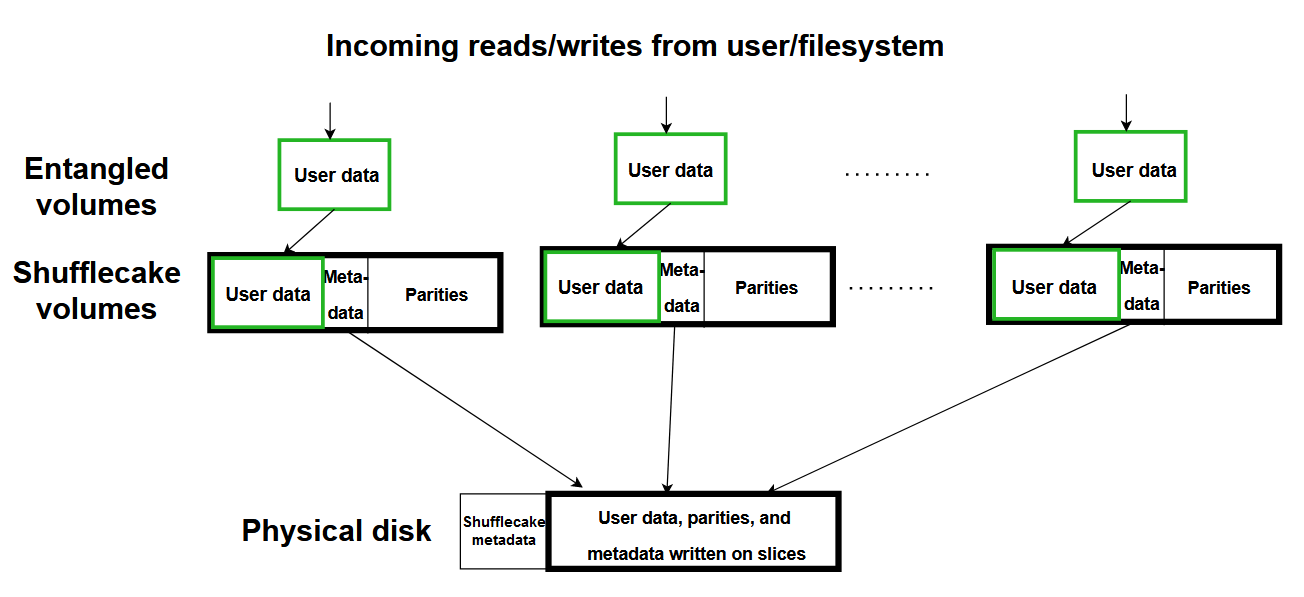
\includegraphics[scale=0.5]{figures/Volumes_diagram.PNG}
    \caption{Depiction of how the virtual volumes are structured}
    \label{fig:volumes-diagram}
\end{figure}

\subsection{Potential issues}
By looking at the diagram on Figure \ref{fig:volumes-diagram}, one might naturally ask how the entanglement metadata is protected from corruption on the physical disk. The answer to that is simple: it is not. Since the entanglement device mapper target works regardless of what the underlying device actually is, it just writes the metadata onto the underlying device. In case of the device being a Shufflecake volume, that same metadata will be written to slices as per the Shufflecake device mapper target. This means that the slices containing the entanglement metadata are susceptible to corruption, much like other data on said slices. One might say a solution is to keep the entanglement metadata together with the metadata of a Shufflecake volume, however the entanglement device mapper target does not know what kind of device is below it. 

Due to the time constraints of this project, this has not been tested, however it is obvious that these metadata blocks are in no way protected on the physical disk. 

\chapter{Results}
To test this implementation, I decided to measure two things: the speed of the write requests, because we change the writing process quite a bit. The goal would be for the user not to be hugely affected by the addition of this tool. The second thing is to check how good the corruption recovery is when faced with different amounts of data corruption, and the time it will take to repair the data. 

For all the testing and debugging purposes, and during the research for this project in general, I used a USB stick of 1GB in size as my underyling block device. More precisely, I partitioned a 32GB USB to make it easier to test and debug, since the whole process would take much longer on the whole 32GB USB. 

\section{Speed of write requests}
For the speed of the write requests, I used the Linux \texttt{dd} \cite{dd_man} and \texttt{time} \cite{time_man} commands. With these commands, I created files filled with random bytes, and wrote them to both the block device directly, and to the block device through my device-mapper target. What this gives us is a clear picture of whether or not the process of creating new parities, calculating checksums, etc. affects the time it takes to write an arbitrary file, if it affects it at all.

I tested my implementation on various workloads, and repeated the test for 30 iterations in order to see the average and the standard deviation of the requests. The results of these tests can be seen in the two tables below. 

\begin{table}[!h]
    \centering
    \begin{tabular}{|c|c|c|c|c|c|c|}
    \hline
       \multicolumn{7}{|c|}{Results from the tests on the block device directly} \\
       \hline
       Workloads  & 1MB & 5MB & 10MB & 50MB & 100MB & 200MB \\
       \hline
       Average write time  & 0.01s & 0.035s & 0.057s & 0.243s & 0.48s & 0.94s \\
       \hline
       Standard deviation  & 0.004 & 0.013 & 0.011 & 0.01 & 0.01 & 0.012 \\
    \hline
    \end{tabular}
    \caption{Time it takes to write a file of a certain size directly onto a block device}
    \label{tab:block_device}
\end{table}

\begin{table}[!h]
    \centering
    \begin{tabular}{|c|c|c|c|c|c|c|}
    \hline
       \multicolumn{7}{|c|}{Results from the tests using the device-mapper target} \\
       \hline
       Workloads  & 1MB & 5MB & 10MB & 50MB & 100MB & 200MB \\
       \hline
       Average write time  & 0.01s & 0.038s & 0.058s & 0.241s & 0.482s & 0.927s \\
       \hline
       Standard deviation  & 0.004 & 0.015 & 0.013 & 0.01 & 0.015 & 0.02 \\
    \hline
    \end{tabular}
    \caption{Time it takes to write a file through the entanglement device-mapper target}
    \label{tab:device_mapper_target}
\end{table}

From these results, we can see that this new entanglement device-mapper target does not impact the performance of write requests from the user. The times for any workload are rather similar, hence have very similar growth patterns as well. This is generally what was desired, to simply have the redundancy scheme working in the background, without the user actually having to sacrifice any time. 

The bash scripts for these particular tests, as well as the results, can be found in the \texttt{speed\_tests} directory of this project. 

\section{Recovery of corrupted data} 
The testing of the actual entanglement algorithm was envisioned as follows. After writing some random files to the device, we would go through the entanglement chain, and randomly corrupt blocks by changing a few bytes of each block. The probability of a block being corrupted would be changed to simulate different loads of data corruption. Time needed to to execute the repair is again measured with the \texttt{time} command. 

Unfortunately, due to the time constraints of this project, and its many changes, these tests have not been done. Most of my time was spent debugging the details regarding the device-mapper target, therefore there was little to no time left for actually testing this. 

\chapter{Conclusion}
In conclusion, adding redundancy to a coercion resistant tool such as Shufflecake proved to be more challenging than anticipated. While the implementation described here could be a solution, there exists the issue mentioned in section 5.1. Choosing the granularity of the implementation proved to be the driving force of this implementation. We tried the idea of working on Shufflecake slices directly, but they are not well suited for entanglements and the algorithm implemented. Therefore, 4KB blocks were the answer. However, working on blocks demands having extra storage overhead, which poses a problem when working with Shufflecake specifically. 

This solution does, however, solve a rather large limitation of previous solutions. Since previous ideas were mirroring blocks and writing them to other slices, there was a probability that writing new blocks might overwrite some sensitive blocks, such as filesystem metadata (superblocks, bitmaps, etc.). Overwriting such files caused the filesystem to crash. By splitting the storage basically in half, as seen in Figure \ref{fig:volumes-diagram} in the "Shufflecake volumes" part, we have solved the issue of the filesystem crashing. Since all the filesystem metadata exists separated from parity blocks, we avoid potentially overwriting some of that metadata when creating new parity blocks. 

I encountered many dead-ends while searching for the solution to this particular problem, and even the solution presented here is not perfect as I have already discussed. However, the idea I explain in the next subsection seems to be the potential solution. 

\section{Further ideas}
Due to all the mentioned issues, the main idea for making Shufflecake more resilient would be to work in the same device mapper target, not create a new one. This way, the necessary per-block metadata can be safely stored, without the risk of being corrupted, and it would be possible to implement a simple entanglement. This idea takes care of the main concerns with the implementation of this redundancy scheme, however it requires major changes to the Shufflecake codebase. Due to the time constraints of this project, this is still just an idea, as there was no time to try and implement it in this way. 

\cleardoublepage
\phantomsection
\addcontentsline{toc}{chapter}{Bibliography}
\printbibliography

% Appendices are optional
% \appendix
% %%%%%%%%%%%%%%%%%%%%%%%%%%%%%%%%%%%%%%
% \chapter{How to make a transmogrifier}
% %%%%%%%%%%%%%%%%%%%%%%%%%%%%%%%%%%%%%%
%
% In case you ever need an (optional) appendix.
%
% You need the following items:
% \begin{itemize}
% \item A box
% \item Crayons
% \item A self-aware 5-year old
% \end{itemize}

\end{document}